\section[Distribuição acumulada]{Função distribuição acumulada}

Considere $A = \left(-\infty, x\right]$, $x \in \R$.
\begin{definition}\label{def:ch02-fda}
    A \textbf{função densidade acumulada} (\fda) é definida como
    \begin{align}
        F(x) &= \Prob(A) = \Prob(-\infty < X \leq x)\label{eq:ch02-fda}
    \end{align}
\end{definition}

\begin{lemma}\label{lem:ch02-fda}
    A \fda\ de uma \va\ $X$ satisfaz às condições:
    \begin{enumerate}
        \item\label{it:ch02-fda-prop-amplitude}
            $0 \leq F(x) \leq 1$
        \item\label{it:ch02-fda-prop-cresc-cd}
            $F(x)$ é uma função não decrescente e contínua à direita
        \item\label{it:ch02-fda-prop-limites}
            $\lim_{x\to -\infty} = 0$ e $\lim_{x\to +\infty} = 1$
    \end{enumerate}
\end{lemma}

\textit{Qualquer} função $F(x)$ \textit{satisfazendo} às condições
\labelcref{it:ch02-fda-prop-amplitude,it:ch02-fda-prop-cresc-cd,it:ch02-fda-prop-limites}
do \cref{lem:ch02-fda} é a \fda\ de alguma \va.

Se $X$ é uma \va\ contínua com \fda\ $F(x)$, então:
\begin{align*}
    \Prob(a < X < b)
    &= \Prob(a \leq X < b) \\
    &= \Prob(a < X \leq b) \\
    &= \Prob(a \leq X \leq b) \\
    &= F(b) - F(a)
\end{align*}

\begin{example}
    A \va\ $X$ tem função densidade
    \begin{align*}
        f(x) &= \begin{cases}
            cx &,\ 0 \leq x \leq \frac{1}{2} \\
            c(1-x) &,\ \frac{1}{2} \leq x \leq 1 \\
            0 &,\ \text{caso contráio}
        \end{cases}
    \end{align*}

    \begin{enumerate}[label=(\alph*)]
        \item Gráfico de $f(x)$.
    \end{enumerate}
    
    \begin{center}
        \begin{tikzpicture}[
            declare function={
                f(\x,\c) = 
                    or(\x<0, \x>1) * 0 +
                    and(\x>=0, \x<=1/2) * (\c*\x) +
                    and(\x>1/2, \x<=1) * (\c*(1 - \x))
                ;}
            ]
            \begin{axis}[
                unbounded coords=jump,
                grid=major,
                axis x line=middle,
                axis y line=middle,
                xmin=-.5, xmax=1.5,
                ymin=0, ymax=1.2,
                xtick={1/2, 1},
                ytick={1},
                xticklabels={$\sfrac{1}{2}$, 1},
                yticklabels={$\sfrac{c}{2}$},
                xlabel={$x$},
                ylabel={$f(x)$},
                y label style={anchor=south},
                x label style={anchor=west},
            ]

            \addplot[blue, ultra thick, samples=5, domain=-1/2:3/2]
                {f(x,2)};

            \end{axis}
        \end{tikzpicture}
    \end{center}

    \begin{enumerate}[label=(\alph*),resume]
        \item Valor de $c$.
    \end{enumerate}
    Temos que
    \begin{align*}
        \int_{=\infty}^{+\infty} f(x)\wrt x
        &= \int_0^1 f(x)\wrt x = 1
    \end{align*}

    Note que a integral acima corresponde à área de um triângulo. Calculamos:
    \begin{align*}
        \int_0^1 f(x)\wrt x &= \frac{1}{2} \cdot \frac{c}{2} \cdot 1 = 1 \\
        \therefore c &= 4
    \end{align*}

    \begin{enumerate}[label=(\alph*),resume]
        \item $F(x)$.
    \end{enumerate}

    Notar que $F(x) = 0$, se $x < 0$ e $F(x) = 1$, se $x > 1$.
    Calculando áreas de triângulos, obtemos
    $F(x) = 2x^2$, se $0 \leq x \leq \frac{1}{2}$
    e $F(x) = 1 - 2(1-x)^2$, se $\frac{1}{2} \leq x \leq 1$.

    \begin{align*}
        F(x) &= \begin{cases}
            0 &,\ x < 0 \\
            2x^2 &,\ 0 \leq x \leq \frac{1}{2} \\
            1 - 2(1-x)^2 &,\ \frac{1}{2} \leq x \leq 1 \\
            1 &,\ x > 1
        \end{cases}
    \end{align*}

    \begin{center}
        \begin{tikzpicture}[
            declare function={
                F(\x) = 
                    (\x<0) * 0 +
                    and(\x>=0, \x<=1/2) * (2*\x^2) +
                    and(\x>1/2, \x<=1) * (1 - 2*(1 - \x)^2) +
                    (\x>1) * 1
                ;}
            ]
            \begin{axis}[
                unbounded coords=jump,
                grid=major,
                axis x line=middle,
                axis y line=middle,
                xmin=-.5, xmax=1.5,
                ymin=0, ymax=1.2,
                xtick={1/2, 1},
                ytick={1/2, 1},
                xticklabels={$\sfrac{1}{2}$, 1},
                yticklabels={$\sfrac{1}{2}$, 1},
                xlabel={$x$},
                ylabel={$F(x)$},
                y label style={anchor=south},
                x label style={anchor=west},
            ]

            \addplot[blue, ultra thick, samples=2, domain=-1/2:0]
                {F(x)};
            \addplot[blue, ultra thick, samples=200, domain=0:1]
                {F(x)};
            \addplot[blue, ultra thick, samples=2, domain=1:3/2]
                {F(x)};

            \end{axis}
        \end{tikzpicture}
    \end{center}

    \begin{enumerate}[label=(\alph*),resume]
        \item $\Prob\left(X > \frac{8}{10}\right)$.
    \end{enumerate}

    Temos que
    \begin{align*}
        \Prob\left(X > \frac{8}{10}\right) 
        &= 1 - \Prob\left(X < \frac{8}{10}\right) \\
        &= 1 - F\left(\frac{8}{10}\right) \\
        &= 1 - \left(1 - 2\cdot\left(1-\frac{8}{10}\right)^2\right) \\
        &= 1 - \frac{23}{25} \\
        &= \frac{2}{25} = 0.08
    \end{align*}

    \begin{enumerate}[label=(\alph*),resume]
        \item $\Prob\left(\frac{1}{4} < X < \frac{3}{4}\right)$.
    \end{enumerate}
    Temos que
    \begin{align*}
        \Prob\left(\frac{1}{4} < X < \frac{3}{4}\right)
        &= F\left(\frac{3}{4}\right) - F\left(\frac{1}{4}\right) \\
        &= \left(1 - 2\cdot\left(1-\frac{3}{4}\right)^2\right)
        - \left(2\cdot\left(\frac{1}{4}\right)^2\right) \\
        &= \frac{7}{8} - \frac{1}{8} \\
        &= \frac{3}{4} = 0.75
    \end{align*}
\end{example}

Se $X$ é uma \va\ contínua e sua função densidade é contínua, 
pelo Teorema Fundamental do Cálculo, temos que
\begin{align}
    F'(x) &= \diff{F}{x} = f(x)\label{eq:ch02-fda-fdp}
\end{align}

Considere agora uma \va\ $X$ discreta com valores no conjunto $\{x_1, x_2,\cdots\}$.
Considere $x \in \R$. Temos:
\begin{align}
    F(x) &= \Prob(-\infty < X < x)
\end{align}

Temos, também, que
\begin{align}
    F(x) &= \sum_{j: x_j \leq x} \Prob(X=x_j)
\end{align}

\begin{example}
    $X\in\{x_1, x_2, x_3, x_4\}$.
    
    \begin{center}
        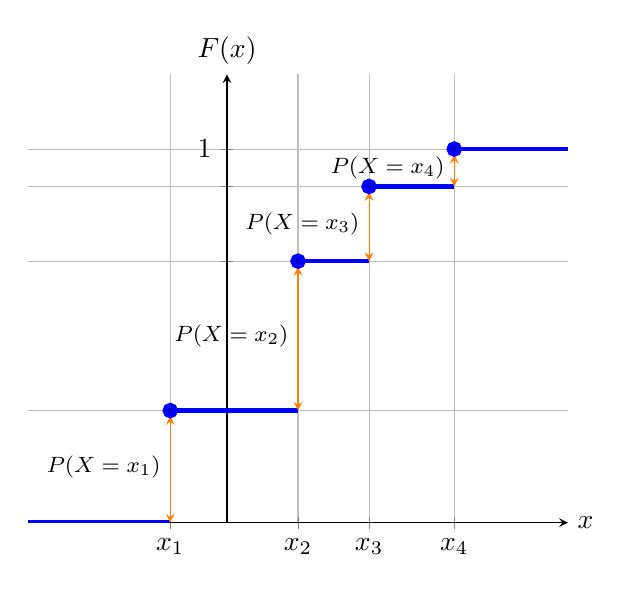
\begin{tikzpicture}[
            declare function={
            F(\x) =
                (\x<-0.4) * 0 +
                (\x>=-0.4) * .3 +
                (\x>=0.5) * .4 +
                (\x>=1.0) * .2 +
                (\x>=1.6) * .1
            ;}
            ]
            \begin{axis}[
                unbounded coords=jump,
                grid=major,
                axis x line=middle,
                axis y line=middle,
                xmin=-1.4, xmax=2.4,
                ymin=0, ymax=1.2,
                xtick={-0.4, 0.5, 1, 1.6},
                ytick={.3,.7,.9,1},
                xticklabels={$x_1$,$x_2$,$x_3$,$x_4$},
                yticklabels={\empty,\empty,\empty,1},
                xlabel={$x$},
                ylabel={$F(x)$},
                y label style={anchor=south},
                x label style={anchor=west},
            ]
                
                \addplot+ [
                    jump mark left,
                    ultra thick,
                    samples at={-1.5, -0.4, 0.5, 1, 1.6, 2.5}
                ] {F(x)};

                \pgfmathsetmacro{\dy}{0.015}
                
                \node[anchor=east] at (-0.4, 0.15) {\footnotesize $P(X=x_1)$};
                \node[anchor=east] at (0.5, 0.5) {\footnotesize $P(X=x_2)$};
                \node[anchor=east] at (1, 0.8) {\footnotesize $P(X=x_3)$};
                \node[anchor=east] at (1.6, 0.95) {\footnotesize $P(X=x_4)$};

                \draw[<->,>=stealth,orange] (-0.4, 0) -- (-0.4, 0.3-\dy);
                \draw[<->,>=stealth,orange] (0.5, 0.3) -- (0.5, 0.7-\dy);
                \draw[<->,>=stealth,orange] (1, 0.7) -- (1, 0.9-\dy);
                \draw[<->,>=stealth,orange] (1.6, 0.9) -- (1.6, 1-\dy);

            \end{axis}
        \end{tikzpicture}
    \end{center}

    \bigskip
    No eixo vertical, a altura das descontinuidades ("saltos") é
    $P(X=x_1)$, $P(X=x_2)$, $P(X=x_3)$ e $P(X=x_4)$, respectivamente.

    Notar que $\lim_{x\to a^+} F(x) = F(a)$.

    \bigskip
    Considere $x_1 \leq x < x_2$.
    
    Neste caso, $F(x) = \Prob(X = x_1)$.

    \bigskip
    Considere, agora, $x_2 \leq x < x_3$.
    
    Neste caso, $F(x) = \Prob(X = x_1) + \Prob(X = x_2)$.

\end{example}

\begin{example}
    \va\ \textbf{mista} (de duas variáveis contínuas).
    \begin{center}
        \begin{tikzpicture}[
            declare function={
            F(\x) =
                1 / (1 + exp(-(\x - 3)/.7))
            ;
            G(\x) =
                0.7 / (1 + exp(-(\x - 3)/1.2))
            ;}
            ]
            \begin{axis}[
                unbounded coords=jump,
                grid=major,
                axis x line=middle,
                axis y line=middle,
                xmin=-1, xmax=6,
                ymin=0, ymax=1.2,
                xtick={3},
                ytick={1},
                xticklabels={$x_0$},
                xlabel={$x$},
                ylabel={$F(x)$},
                y label style={anchor=south},
                x label style={anchor=west},
            ]

                \addplot[blue, ultra thick, samples=100, domain=3:7]
                    {F(x)};
                \addplot[blue, only marks, ultra thick, samples at={3}]
                    {F(x)};
                \addplot[blue, ultra thick, samples=100, domain=-1:3]
                    {G(x)};
                \addplot[blue, fill=white, only marks, ultra thick, samples at={3}]
                    {G(x)};

                

            \end{axis}
            \end{tikzpicture}
    \end{center}    
\end{example}

\begin{notation}
    A notação $f(x_0^-)$ indica que a função $f$ foi avaliada
    num ponto muito próximo de $x_0$ pelo lado esquerdo, ou seja,
    em valores menores que $x_0$. Em outras palavras:
    \begin{align*}
        f(x_0^-) &= \lim_{x \to x_0^-} f(x) \\
            &= \lim_{x \upto x_0^-} f(x) \\
            &= \lim_{\epsilon \to 0^+} f(x - \epsilon) \\
            &= \lim_{\epsilon \downto 0} f(x - \epsilon)
    \end{align*}
\end{notation}

\begin{example}
    $X$ é um \va\ discreta com \fda\ $F(x)$. Considere $a < b$.

    Calcular, usando $F(x)$:
    
    \begin{enumerate}
        \item $\Prob(a < X < b)$
    \end{enumerate}

    Notar que
    \begin{align*}
        \left(-\infty, b\right)
        &= \left(-\infty, a\right] \cup \left(a, b\right)
    \end{align*}

    Calculando as probabilidades, obtemos
    \begin{align*}
        \Prob(-\infty < X < b)
        &= \Prob(-\infty < X \leq a)
        + \Prob(a < X < b) \\
        \implies F(b^-) &= F(a) + \Prob(a < X < b)
    \end{align*}
    
    Ou, seja,
    \begin{align*}
        \Prob(a < X < b) &= F(b^-) - F(a)
    \end{align*}
    
    \begin{enumerate}[resume]
        \item $\Prob(a \leq X < b)$
    \end{enumerate}

    Notar que
    \begin{align*}
        \left(-\infty, b\right)
        &= \left(-\infty, a\right) \cup \left[a, b\right)
    \end{align*}

    Calculando as probabilidades, obtemos
    \begin{align*}
        \Prob(-\infty < X < b)
        &= \Prob(-\infty < X < a)
        + \Prob(a \leq X < b) \\
        \implies F(b^-) &= F(a^-) + \Prob(a \leq X < b)
    \end{align*}
    
    Ou, seja,
    \begin{align*}
        \Prob(a \leq X < b) &= F(b^-) - F(a^-)
    \end{align*}
    
    \begin{enumerate}[resume]
        \item $\Prob(a < X \leq b)$
    \end{enumerate}

    Notar que
    \begin{align*}
        \left(-\infty, b\right]
        &= \left(-\infty, a\right] \cup \left(a, b\right]
    \end{align*}

    Calculando as probabilidades, obtemos
    \begin{align*}
        \Prob(-\infty < X \leq b)
        &= \Prob(-\infty < X \leq a)
        + \Prob(a < X \leq b) \\
        \implies F(b) &= F(a) + \Prob(a < X \leq b)
    \end{align*}
    
    Ou, seja,
    \begin{align*}
        \Prob(a < X \leq b) &= F(b) - F(a)
    \end{align*}

    \begin{enumerate}[resume]
        \item $\Prob(a \leq X \leq b)$
    \end{enumerate}

    Notar que
    \begin{align*}
        \left(-\infty, b\right]
        &= \left(-\infty, a\right) \cup \left[a, b\right]
    \end{align*}
    
    Calculando as probabilidades, obtemos
    \begin{align*}
        \Prob(-\infty < X \leq b)
        &= \Prob(-\infty < X < a)
        + \Prob(a \leq X \leq b) \\
        \implies F(b) &= F(a^-) + \Prob(a \leq X \leq b)
    \end{align*}
    
    Ou, seja,
    \begin{align*}
        \Prob(a \leq X \leq b) &= F(b) - F(a^-)
    \end{align*}

    Sumarizando os resultados acima, obtemos:
    \begin{center}
        \begin{tabular}{cl}
            \toprule
             $\Prob(a < X < b)$       & $F(b^-) - F(a)$   \\
             $\Prob(a \leq X < b)$    & $F(b^-) - F(a^-)$ \\
             $\Prob(a < X \leq b)$    & $F(b) - F(a)$     \\
             $\Prob(a \leq X \leq b)$ & $F(b) - F(a^-)$   \\
             \bottomrule
        \end{tabular}
    \end{center}
\end{example}

\begin{example}
    Considere $X\in\{x_1, x_2, x_3, x_4\}$.
    
    Seja $a \in (x_2, x_3)$ e $b = x_4$.

    \begin{center}
        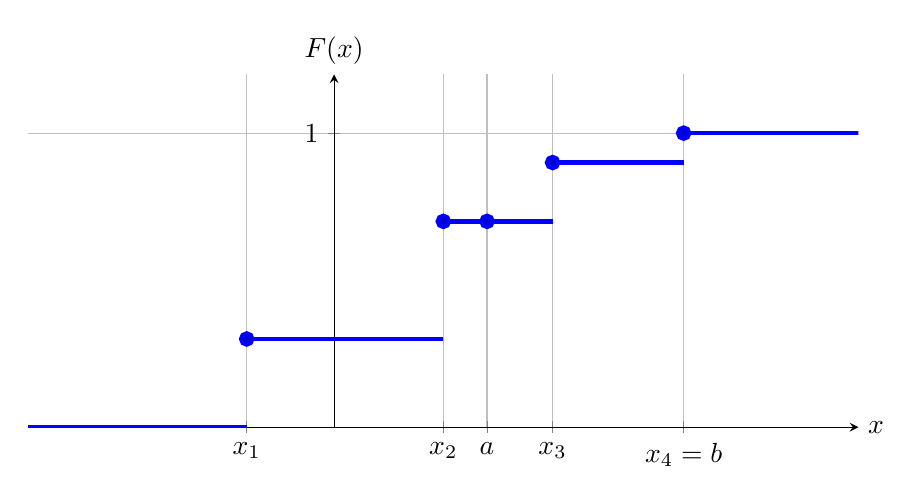
\begin{tikzpicture}[
            declare function={
            F(\x) =
                (\x<-0.4) * 0 +
                (\x>=-0.4) * .3 +
                (\x>=0.5) * .4 +
                (\x>=1.0) * .2 +
                (\x>=1.6) * .1
            ;}
            ]
            \begin{axis}[
                unbounded coords=jump,
                grid=major,
                axis x line=middle,
                axis y line=middle,
                xmin=-1.4, xmax=2.4,
                ymin=0, ymax=1.2,
                xtick={-0.4, 0.5, 0.7, 1, 1.6},
                ytick={1},
                xticklabels={$x_1$,$x_2$,$a$,$x_3$,$x_4 = b$},
                xlabel={$x$},
                ylabel={$F(x)$},
                y label style={anchor=south},
                x label style={anchor=west},
                width=\textwidth,
                height=0.5\textwidth,
            ]
                
                \addplot+ [
                    blue,
                    jump mark left,
                    ultra thick,
                    samples at={-1.5, -0.4, 0.5, 0.7, 1, 1.6, 2.5}
                ] {F(x)};

            \end{axis}
        \end{tikzpicture}
    \end{center}

    \begin{align*}
        \Prob(a < X < b) &= F(b^-) - F(a) \\
        &= F(x_4^-) - F(a) \\
        &= F(x_3) - F(x_2) \\
    \end{align*}

    \begin{obs}
        Sem usar a \fda, temos
        \begin{align*}
            \Prob(a < X < b) &= \sum_{a < x < b} \Prob(X =x)
        \end{align*}
    \end{obs}
\end{example}